% ===================================================================================================
\chapter{Simulations}
% ===================================================================================================

The molecular dynamics code used in this work was the Large-scale Atomic/Molecular Massively Parallel Simulator (LAMMPS) developed by Sandia National Laboratories \cite{lammpsMD}. 
LAMMPS is a free and open-source code, which utilises the Message Passing Interface (MPI) for running spatially-decomposited parallel MD simulations.
Additionally, LAMMPS also provides a scripting language used to set input parameters and run simulations, but which also contains tools for creating and manipulating simple simulation cells.    

The interatomic potential of choice for our simulations was the W-H-He EAM potential developed by Bonny \textit{et al.} and referred to as 'EAM1' in \cite{bonny2014binding}. 
The W-W interaction part of this potential is the same as in 'EAM2' developed by Marinica \textit{et al.} in \cite{marinica2013interatomic}. 
It is well-known for providing elastic constants as well as point defect, dislocation and grain boundary properties in good agreement with Density Functional Theory (DFT) calculations and experiments \cite{bonny2014many}. 
The W-H-He potential referred hereafter to as just 'EAM1', has been shown to relatively accurately recreate the interactions of H with both point defects and dislocations in W \cite{bonny2014binding, grigorev2015interaction}. 

Due to the long in-simulation times, particular attention had to be paid to optimisation of all aspects of the simulations.
The overall computational load could be reduced by scaling down the atomic systems to the bare minima without significantly affecting the accuracy of our results.
For instance, by reducing the side length of a cubic cell of tungsten from 12 unit cells to 10, we have exactly 662 fewer atoms. 
Assuming a linear, $O(N)$ time complexity, this amounts to a 25 \% decrease in wall-time.
On a two-week-long parallel simulation run on six CPUs, this small change would mean saving over 500 CPU hours. 

For systems consisting of thousands of atoms, running MD in parallel is imperative, but comes with additional considerations.  
Utilising too few CPUs results in obvious performance issues, while using too many is wasteful and can cause slow-downs due to increased inter-processor communication.
A poorly chosen number of CPUs can additionally result in a suboptimal division of the simulation cell among the processors. 
By using short test runs, we could determine the optimal number of CPUs for each configuration.

% ---------------------------------------------------------------------------------------------------
\section{Simulation Setups}
% ---------------------------------------------------------------------------------------------------
Although the simulations differ largely from defect to defect, a general pattern can be extracted for all of our isotope exchange simulations. 
First, a simulation cell of bulk W containing the defect was created and allowed to reach a minimum energy configuration by first employing numerical minimization and then relaxation through repeatedly heating and cooling the system during short MD cycles. 
The energy minimization method of choice was a Polak-Ribi\`{e}re conjugate gradient algorithm \cite{polak1969note}, which iteratively shifts atom coordinates until a local energy minimum is reached. 

Following the initial relaxation, a large amount of T atoms were deposited at random positions around the cell and allowed to diffuse around during successive MD runs, until the defect had been fully saturated with hydrogen.
After this, the excess T was removed before adding H to random interstitial sites around the cell. 
Isotope exchange was then simulated by running MD until the tritium was completely removed from the defect.
In practice, this amounted to total simulation times of 100...3000 ns and wall-times of 1...4 months depending on the defect type in question. 

Periodic boundaries were applied in all directions, and the pressure and temperature were controlled using Nos\'{e}-Hoover thermostats and barostats, emulating an isothermal-isobaric ensemble. 
In a real-world situation, a T atom leaving a defect and diffusing far away would very unlikely return to its starting point, as opposed to getting caught in another defect or leaving the material through a surface. 
Due to the periodic boundaries, however, the T atoms cannot leave the space defined by the cell, as a border-crossing atom merely returns from the opposite side. 
The simulations were therefore performed in intervals of 5 ps (5000 time steps), and after each interval, any T atoms having moved sufficiently far away were automatically removed from the simulation. 
In this scope, 'far away' was defined as a distance $d_{\rm{rmv}} $ from the initial position of the T atom. 
Depending on the geometry of the defect, this parameter had a value of 14...40 \AA, i.e. ca 4...13 unit cells.

As we intend to verify that isotope exchange indeed results in more effective tritium removal than conventional methods, setups for comparison simulations were constructed by omitting the added H and only simulating the spontaneous diffusion of T away from the defect. 
These monoisotopic systems are used for emulating vacuum annealing conditions.

Finally, all sets of isotope exchange and monoisotope simulations were run at 400, 500 and 700 K, to qualitatively and semi-quantitatively study the temperature dependence of the phenomenon.
To allow for shorter wall-times, the simulations where cut off when all T had been detrapped in the isotope exchange case.  


% --------------- IsoEx MD ------------------------------------------------------------------------------------
\begin{figure}[!ht]
\begin{center}
% Define block styles
\tikzset{
decision/.style = {diamond, draw, fill=green!40, 
    text width=4.5em, text badly centered, node distance=3cm, inner sep=0pt},
block/.style = {rectangle, draw, fill=cyan!30, 
    text width=12em, text centered, rounded corners, minimum height=1.5em},
smallblock/.style = {block, text width=7em},
cloud/.style = {draw, ellipse,fill=red!20, node distance=3cm,
    minimum height=1.5em}
    }
\begingroup  % compress equations
\medmuskip=2mu
\thinmuskip=1mu
\thickmuskip=2mu
\begin{tikzpicture}
\matrix (m)[matrix of nodes, column  sep=0.0cm,row  sep=5mm, align=center, nodes={rectangle,draw, anchor=south} ]{
   |[block] (initI)| {\small Create simulation cell containing defect} & \\
   |[block] (initII)| {\small Relax and Deposit H} & \\
    |[block] (MD)| {\small Run MD for 5000 steps}          &  \\
    |[block] (DelT)| {\small Delete T atoms for which $d_i > d_{\text{rmv}}$}          &  \\
%    |[block] (Calcd)| {Calculate $d_i$}          &  \\
%    |[decision] (IsOut)| {$d_i > d_{\rm{rmv}}$?}              &  \\
%       & |[smallblock] (Rmv)| {Remove $i$th T}         &  \\
   |[decision] (IsEnd)| {\small End condition reached?}              &  \\
   |[block] (End)| {\small Save results and quit}   & \\
};
\path [>=latex,->] (initI) edge (initII);
\path [>=latex,->] (initII) edge (MD);
\path [>=latex,->] (MD) edge (DelT);
\path [>=latex,->] (DelT) edge (IsEnd);
%\path [>=latex,->] (MD) edge (Calcd);
%\path [>=latex,->] (Calcd) edge (IsOut);
%\draw [>=latex,->] (IsOut.east) -| node[above, near start] {yes} (Rmv.north);
%\draw [>=latex,->] (IsOut.south) -- node[right] {no}(IsEnd);
%\draw [>=latex,->] (Rmv.south) |- (IsEnd.north);
\draw [>=latex,->] (IsEnd.west) -- node[above] {no} ++(-2,0cm) |- (MD.west);
\draw [>=latex,->] (IsEnd.south) -- node[right] {yes}(End);
\end{tikzpicture}
\endgroup
\caption{A flowchart representation of the isotope exchange simulations. Variable $d_i$ refers to the distance between current and initial point of T atom $i$.} 
\label{Fig:isoExSimus}
\end{center}
\end{figure}


% ---------------------------------------------------------------------------------------------------
\subsection{Vacancies}
% ---------------------------------------------------------------------------------------------------
For the vacancy simulations, a monovacancy was created by removing the middlemost atom of a $10\times 10 \times 10$ unit cell (2000 atom) W lattice.  
In contrast to the larger systems, where the defect was saturated using random diffusion, the small size of the point defect enabled us to manually place T at their natural lowest energy positions.
These positions coincide with the octahedral interstitial sites, forming a square bipyramid around the vacancy \cite{heinolaTungstenDFT}.
A total of 19 H atoms were then deposited to randomly chosen tetrahedral interstitial sites around the simulation W lattice, as seen in Fig. \ref{Fig:monovac_system}, bringing the (H+T)/W ratio to 0.0125. 

A divacancy system was constructed in a similar fashion by removing two neighbouring W atoms and adding a total of 10 T atoms to the defect.
The (H+T)/W ratio in these simulations was 0.0150.

\begin{figure}[!ht]
\center
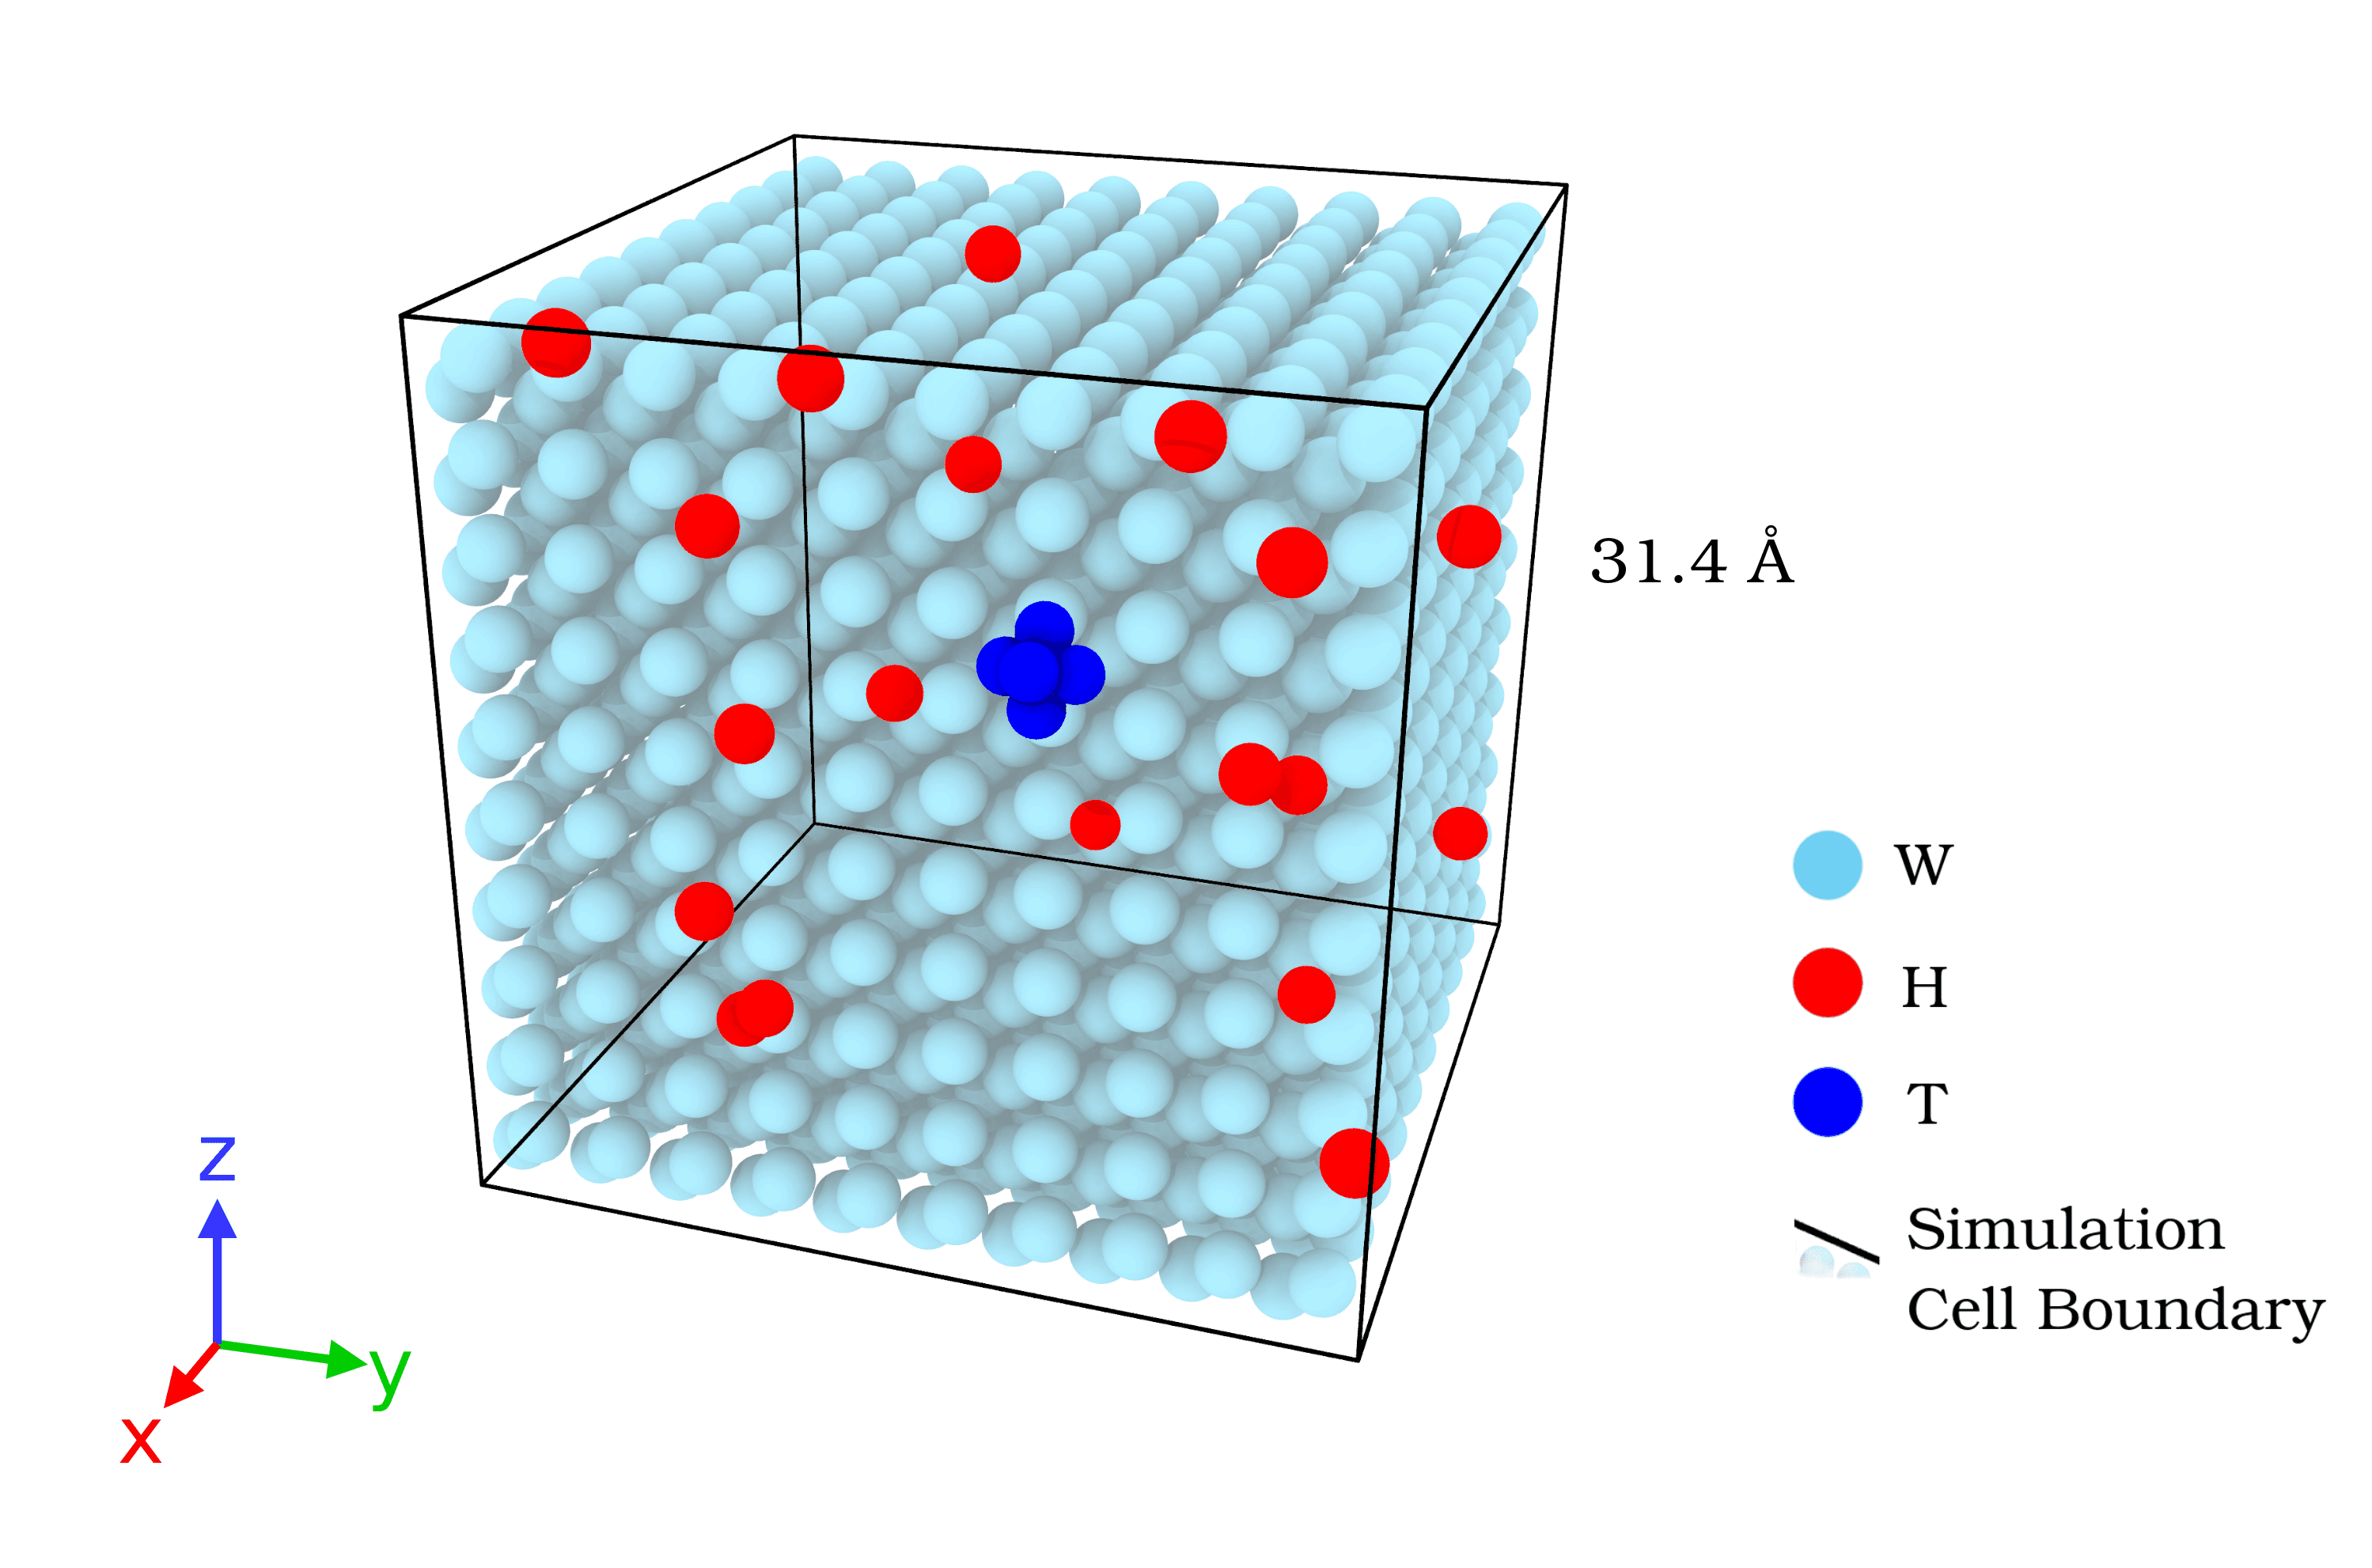
\includegraphics[width=0.7\linewidth]{1Vac_system.png}
\caption{The initial state of the simulation cell used in the monovacancy simulations. 
The W atoms are rendered translucent to display the positions of the hydrogen isotopes.}
\label{Fig:monovac_system}
\end{figure}

% ---------------------------------------------------------------------------------------------------
\subsection{Dislocations}
% ---------------------------------------------------------------------------------------------------
For the dislocation simulations, a  $109.0 \times 136.8 \times 18.4$ $\AA^3$ simulation cell containing an arbitrarily chosen 1/2\hkl[1 1 1]\hkl{1 0 0} edge dislocation was used. 
The defect was generated by first producing a cuboid supercell, with the $x$, $y$ and $z$ axes oriented along the crystal directions \hkl[1 1 1], \hkl[1 1 -2] and \hkl[-1 1 0], respectively, as shown in Fig. (\ref{Fig:disloc_system}). 
The cell was then divided into three equally thick slices, parallel to the \hkl{11-2} plane and a dislocation was introduced by inserting a redundant \hkl{1 1 1} atom plane to the middlemost slice, as shown in Fig. \ref{Fig:disloc_construction}. 
In order to facilitate the formation of a natural dislocation and to enable the use of periodical boundary conditions, the atom positions in the middle slice were finally compressed slightly.

\begin{figure}[!ht]
\center
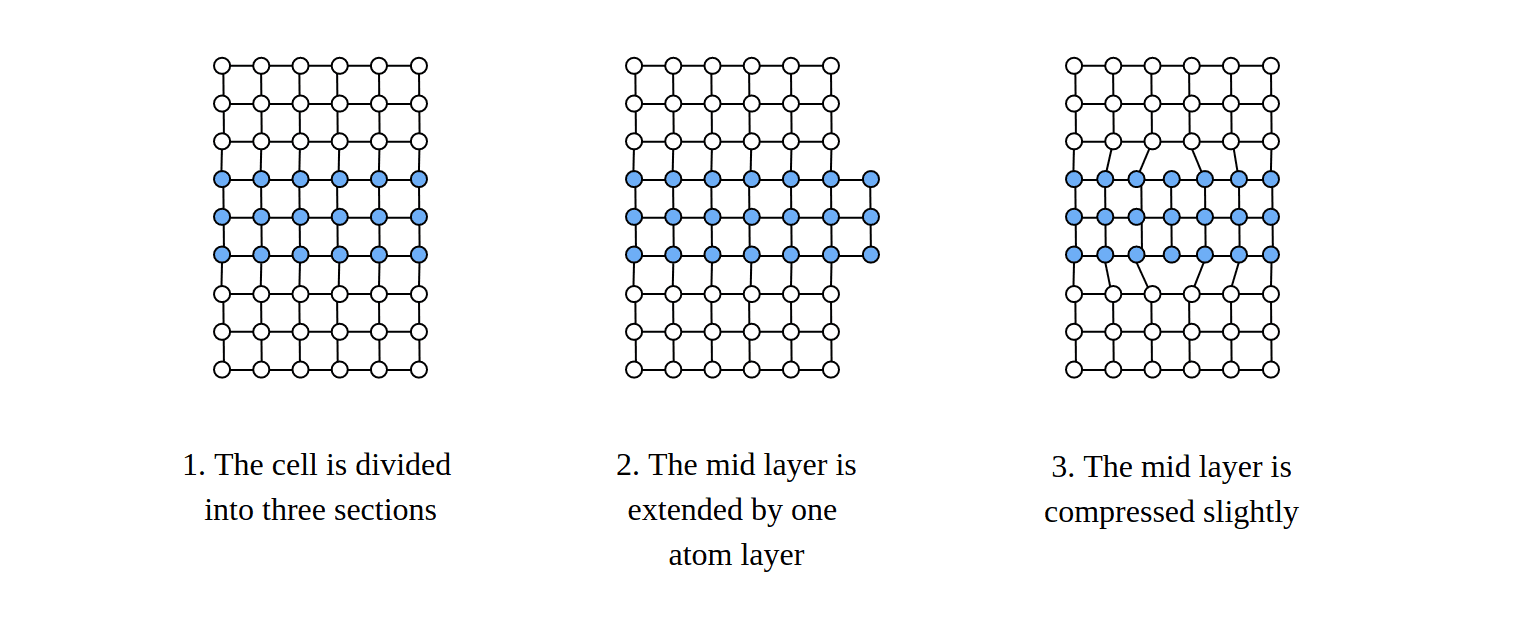
\includegraphics[width=0.85\linewidth]{disloc_construction.png}
\caption{A 2D sketch of the process of constructing the dislocation supercell}
\label{Fig:disloc_construction}
\end{figure}

In practice, the simulation cell was generated using Atomsk \cite{hirel2015atomsk}, an open-source command-line tool for creating and manipulating data files for atomistic simulations.
With the bulk tungsten cell consisting of 17 424 atoms, the dislocation containing 132 T atoms after saturation and 150 H atoms having been added to random locations, the (H+T)/W ratio was brought to 0.016. 

\begin{figure}[!ht]
\center
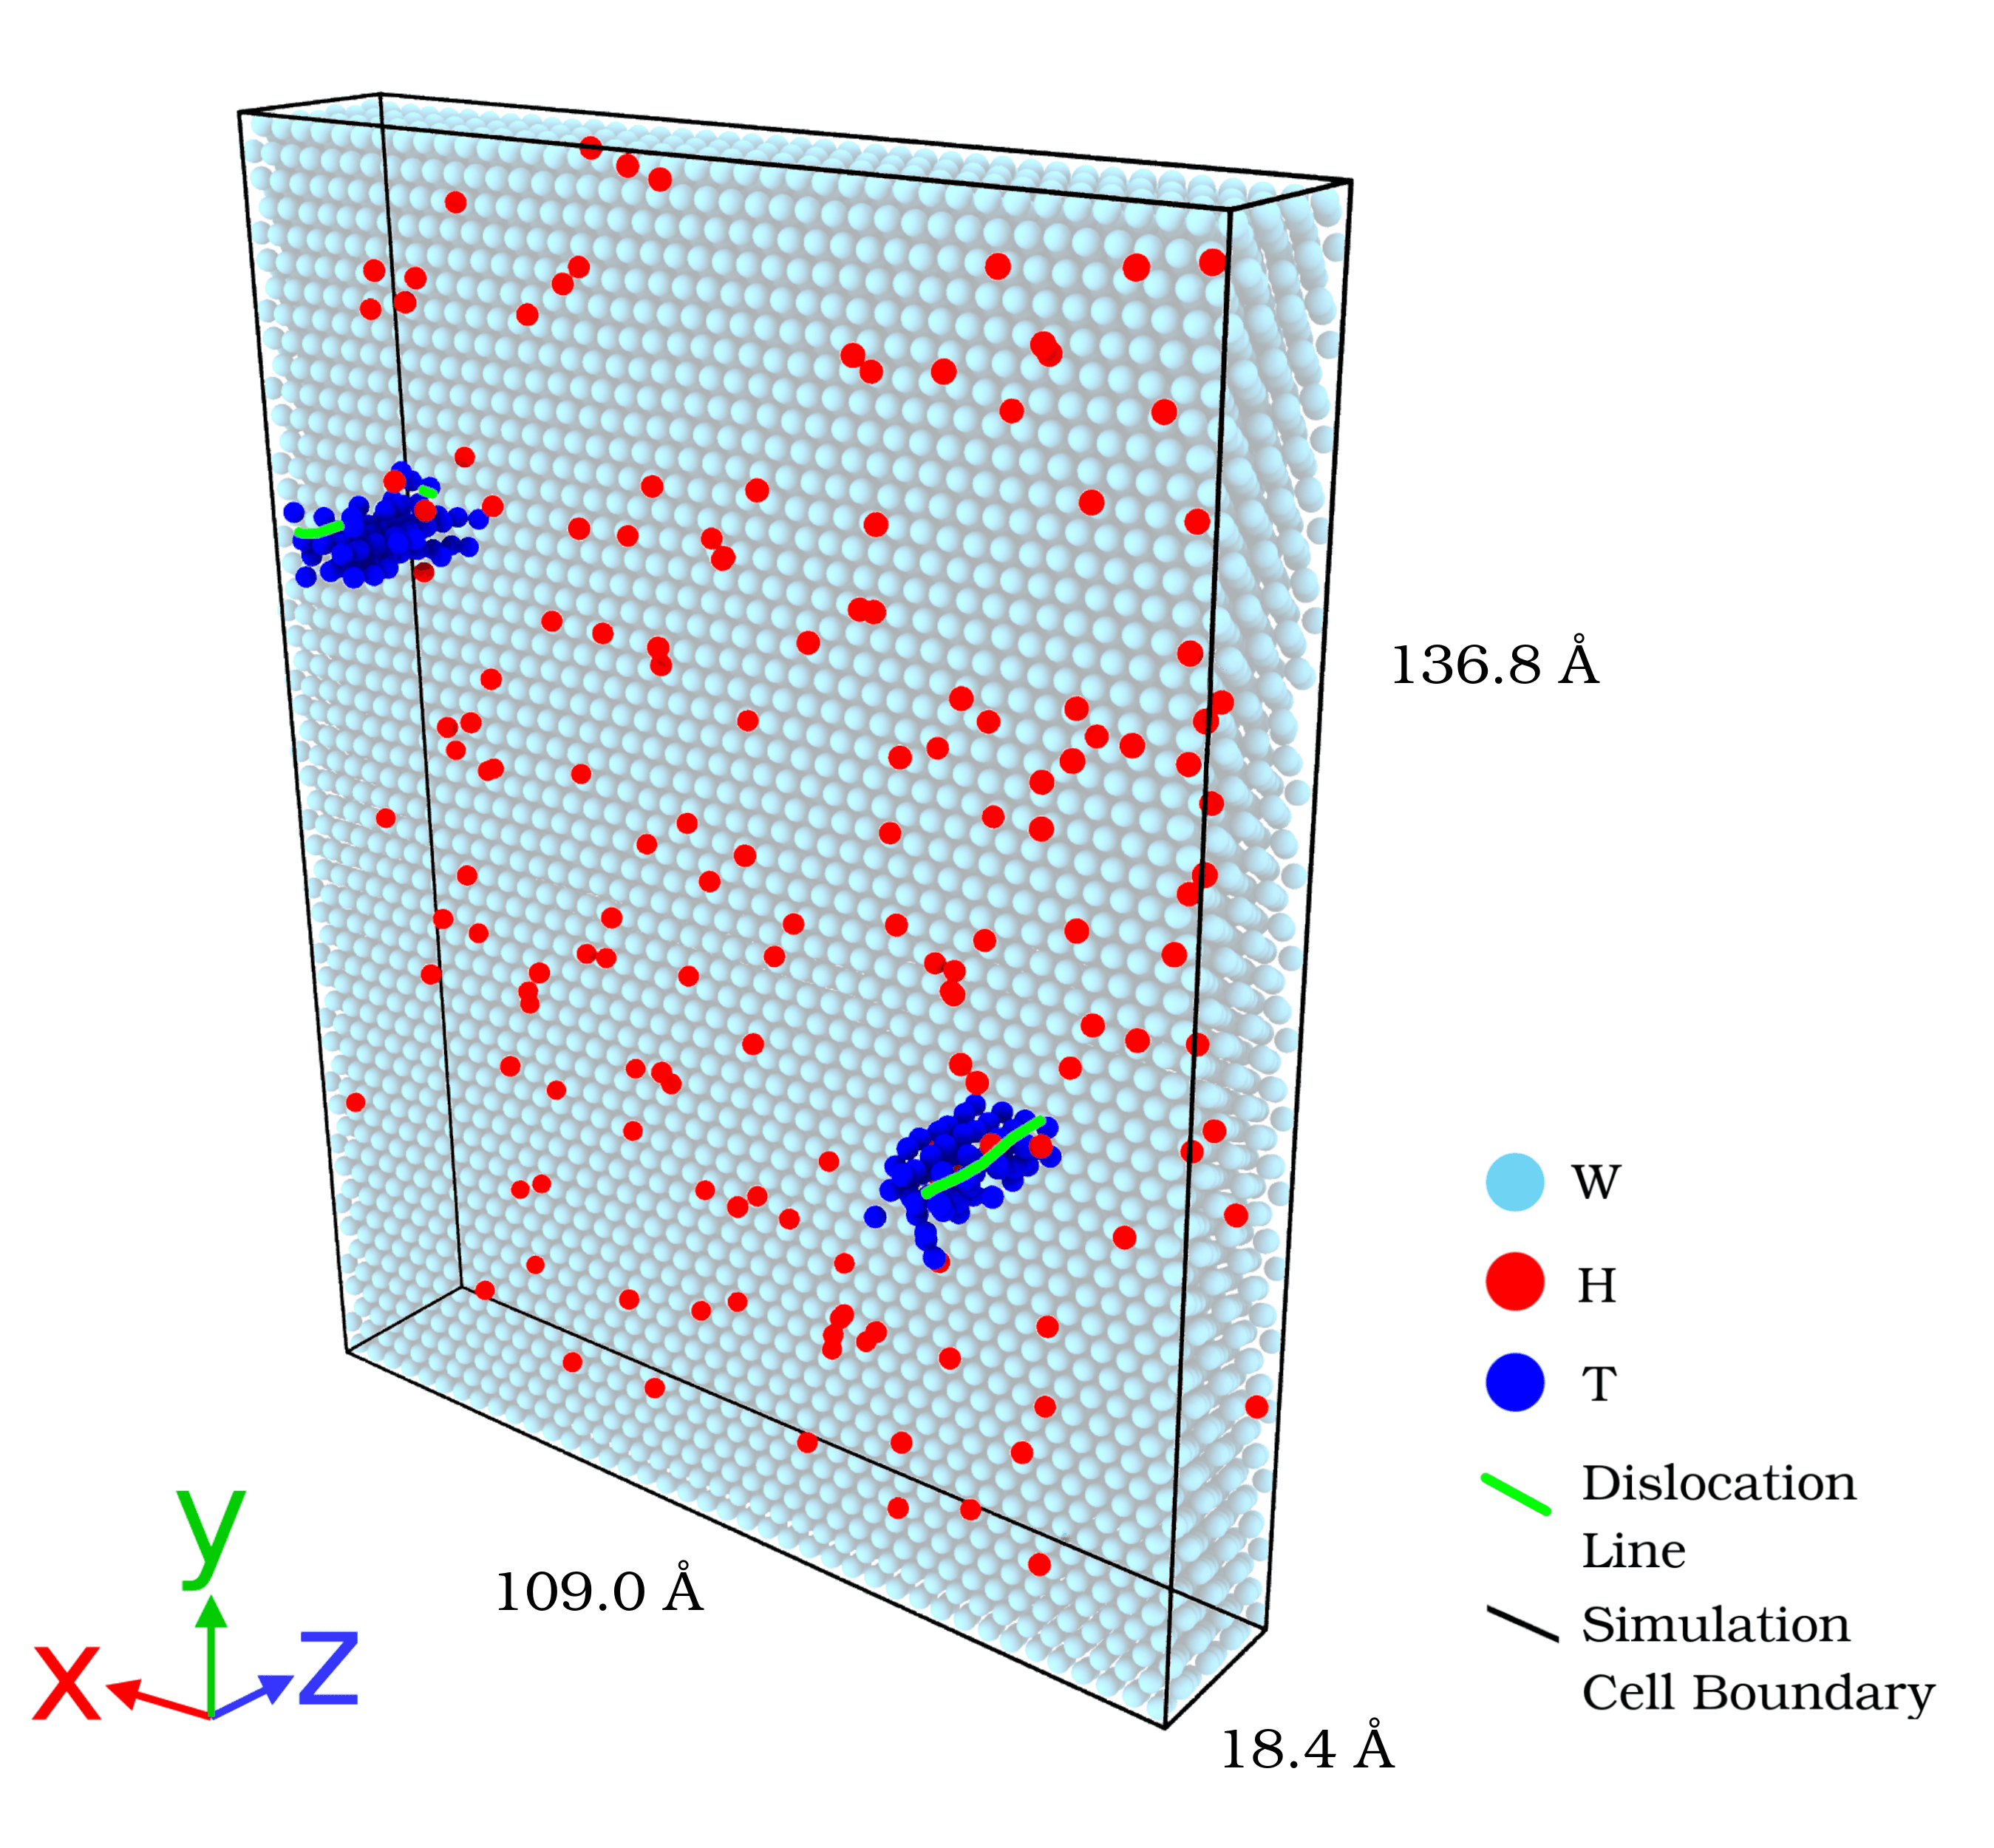
\includegraphics[width=0.7\linewidth]{disloc_system.png}
\caption{The initial state of the simulation cell used in the dislocation simulations. 
The W atoms are rendered translucent to display the positions of the hydrogen isotopes. 
The dislocation, together with its periodic images, is visualized using a defect mesh.}
\label{Fig:disloc_system}
\end{figure}

% ---------------------------------------------------------------------------------------------------
\subsection{Grain Boundaries}
% ---------------------------------------------------------------------------------------------------
% $\Sigma$5\hkl{310}/\hkl[001]
For simulating isotope exchange in W grain boundaries, we used a system containing an arbitrarily chosen \hkl(310)\hkl[001] tilt grain boundary. 
The simulation cell was created by growing together two separate tungsten lattices, each rotated through $\pm18.43^\circ$, respectively, around the $z$-axis. 
As the $x$-axes of the lattices point along \hkl<310> directions, we have a system with a periodicity of $\sqrt{10}~a$ along the $x$- and $y$-axes, and $a$ along the $z$-axis. 
In order to minimize the number of atoms needed to simulate the system we can set $y >> x \approx z$ and again use periodic boundaries.

% Zhou_2009_H_behaviour_in_W_grain_boudnary_FP.pdf

The data file describing the simulation cell was created using Atomsk \cite{hirel2015atomsk} to grow out the intersecting lattices of the two grains from predefined starting points. 
Overlapping W atoms were later manually removed to produce a clean \hkl(310)\hkl[001] grain boundary.
Due to the size and shape of the simulation cell, it contained 30002 W atoms and 73 T atoms were bound to the grain boundary during saturation.
After deposition 150 H atoms, the (H+T)/W ratio was 0.0576.

\begin{figure}[!ht]
\center
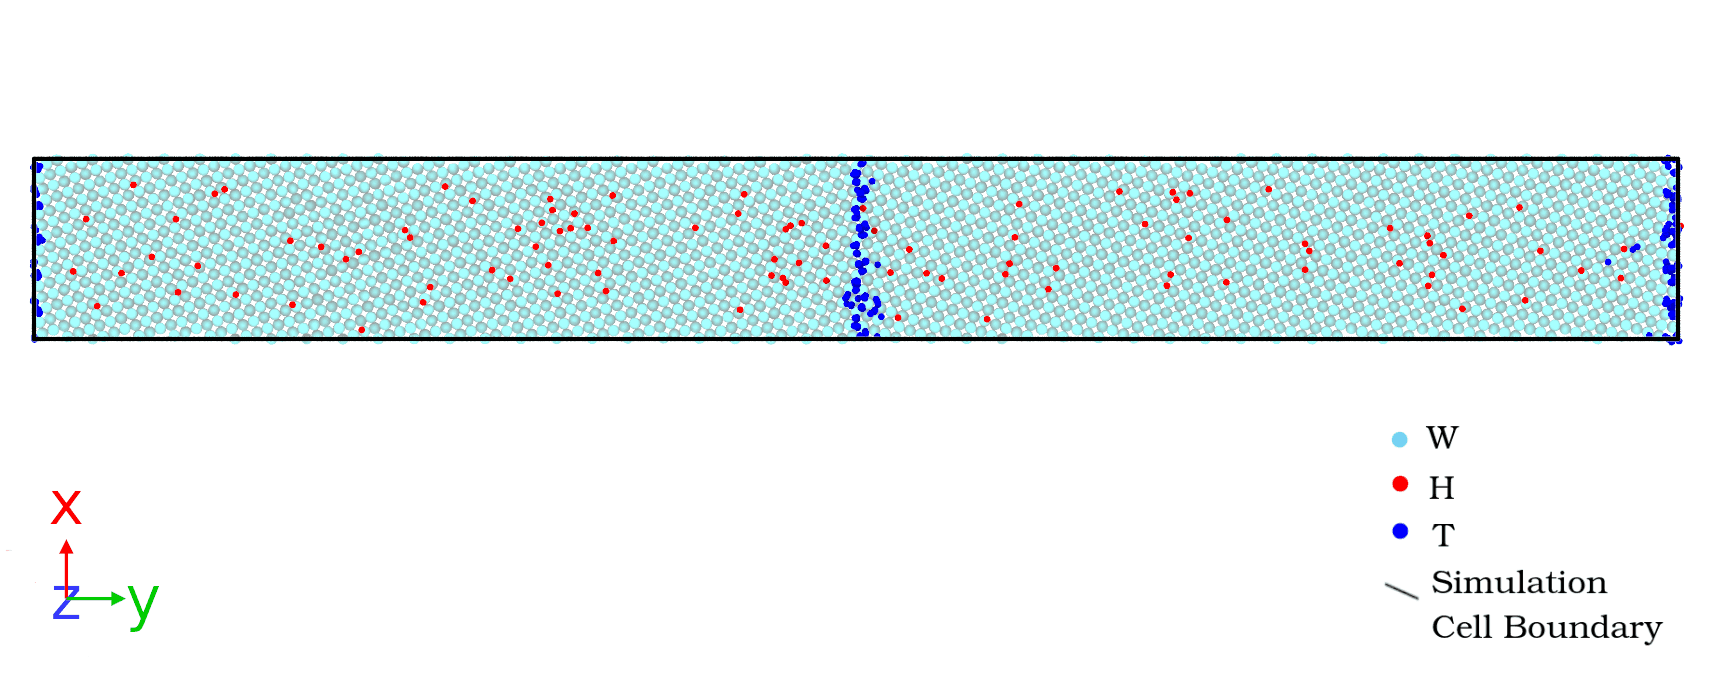
\includegraphics[width=0.94\linewidth]{GB_system.png}
\caption{The initial state of the simulation cell used in the grain boundary simulations. 
The W atoms are rendered translucent to display the positions of the hydrogen isotopes. Break lines are shown to indicate that the cell has been shortened for visual purposes}
\label{Fig:GB_system}
\end{figure}

% ---------------------------------------------------------------------------------------------------
\section{Data Analysis}
% ---------------------------------------------------------------------------------------------------

For each successful simulation, two coordinate dump files were produced, one containing the coordinates of the H and T atoms every 250 time steps ($2.5\cdot 10^{-4}$ ns) and another with the W atom coordinates every $5\cdot 10^5$ time steps (0.5 ns).
Since the motion of the defects themselves was practically negligible, the number of H and T bound to a defect could be determined by defining a geometric region in space around the defect and overlaying this region with each frame of the H-T dump file.

In practice, this was performed by parsing the dump files with a Fortran program, which checked whether each atom was located inside or outside the specified region and outputted the numbers of H and T in the defect as functions of time.

As a means of comparing the T-removal rates between defects, we can use normalised average removal rates calculated as
\begin{align}
\delta_{\text{T}} = \frac{\left(N_{\text{T}}^{\text{initial}}-N_{\text{T}}^{\text{final}}\right)/N_{\text{T}}^{\text{initial}}}{\Delta t}
\label{Eq:AverageRemovalRate}
\end{align}
where $N_{\text{T}}^{\text{initial}}$ is the initial number of T in the defect and $\Delta t$ is the time passed in nanoseconds while removing $N_{\text{T}}^{\text{initial}}-N_{\text{T}}^{\text{final}}$ atoms.

